\documentclass[12pt]{article}

\newcommand{\reporttitle}{Adaptive 1D 1st-order Lagrange FEM}
\newcommand{\accentcolor}{solarized-green}
\newcommand{\urlcolor}{solarized-red}

\usepackage{amsmath}
\usepackage{amsthm}
\usepackage{amsfonts}
\usepackage{amssymb}

\newcommand{\R}{\mathbb{R}}
\newcommand{\N}{\mathbb{N}}

\newtheorem{theorem}{Theorem}

\usepackage{courier}
\usepackage{listings}

\lstdefinestyle{default}{
	commentstyle=\color{solarized-green},
	keywordstyle=\color{solarized-magenta},
	stringstyle=\color{solarized-purple},
	basicstyle=\ttfamily\color{solarized-base02},
	breakatwhitespace=false,
	breaklines=true,
	captionpos=b,
	keepspaces=true,
	numbersep=5pt,
	showspaces=false,
	showstringspaces=false,
	showtabs=false,
	tabsize=2
}

\lstset{style=default}

\usepackage{nameref}

\usepackage{titlesec}

\usepackage{graphicx}
\graphicspath{{../gallery/}}

\usepackage{xcolor-solarized}
\usepackage{pagecolor}
\color{solarized-base02}

\usepackage[T1]{fontenc}
\usepackage[utf8]{inputenc}

\usepackage[a4paper]{geometry}
\geometry{
	inner=20mm,
	outer=20mm,
	top=30mm,
	bottom=30mm,
	heightrounded,
	marginparwidth=50pt,
	marginparsep=20pt,
	headsep=25pt,
	headheight=30pt
}

\usepackage{hyperref}
\hypersetup{
	linktocpage=true,
	colorlinks=true,
	linkcolor=\accentcolor,
	urlcolor=\urlcolor,
	pdftitle={\reporttitle},
	pdfpagemode=FullScreen,
	pdfauthor={Andrea Di Antonio}
}

\usepackage{fancyhdr}
\pagestyle{fancy}
\fancyhf{}
\fancyhead[R]{Andrea Di Antonio}
\fancyhead[L]{\reporttitle}
\fancyfoot[C]{\thepage}

\title{\reporttitle}
\author{Andrea Di Antonio, 858798 \\ \hyperlink{mailto:a.diantonio1@campus.unimib.it}{a.diantonio1@campus.unimib.it}}
\date{Exam session of July 27, 2023 \\ Academic Year 2022-23}

\setcounter{tocdepth}{2}

\begin{document}
	\pagenumbering{roman}
	\maketitle
	\thispagestyle{fancy}

	\begin{abstract}
		\begin{center}
			Report for the course \textit{Metodi Numerici per Equazioni alle Derivate Parziali} on the definition and costruction of an \textit{\reporttitle}\footnote{Written in MATLAB, R2023b.} and a subsequent analysis which includes a comparison against a more naive approach by considering a sequence of uniformly refined meshes.
		\end{center}
	\end{abstract}

	\newpage
	\tableofcontents

	\newpage
	\pagenumbering{arabic}
	\section{Problem Introduction}
	\subsection{Poisson Problem}

Let's start by considering the following problem, given $\Omega = (0, 1)$:
\begin{gather}
	\begin{cases}
		-u^{\prime \prime}(x) = f(x) \quad \text{in } \Omega \\
		u(0) = u(1) = 0
	\end{cases},
\end{gather}
which is the \textit{Poisson equation} on $\Omega$ with \textit{Dirichlet's boundary conditions}.

We'll consider a source $f(x)$ evaluated by considering the exact solution $u_{\alpha}$:
\begin{gather}
	u_{\alpha}(x) = x^{\alpha} (1 - x),
\end{gather}
on $\alpha > 1.5$, so that:
\begin{gather}
	f(x) = \alpha (\alpha + 1) x^{\alpha - 1} - \alpha (\alpha - 1) x^{\alpha - 2}.
\end{gather}

\subsubsection{Solution's Sobolev Regularity}

% To be discussed

\subsection{Weak Formulation and Finite Element Discretization} \label{fem_definition}

The weak formulation for the problem requires to find a $u \in V = H_0^1(\Omega)$ such that:
\begin{gather}
	a(u, v) = (f, v)_{0, \Omega} \quad \forall v \in V,
\end{gather}
where:
\begin{gather}
	a(u, v) = (u^{\prime}, v^{\prime})_{0, \Omega}.
\end{gather}

By introducing $V_h$ as the linear Lagrangian finite element space on a given partition $T_h$ of $\Omega$ we have the finite element discretization which requires to find a $u_h \in V_h$ such that:
\begin{gather}
	a(u_h, v_h) = (f, v_h)_{0, \Omega} \quad \forall v_h \in V_h,
\end{gather}

	\newpage
	\section{Finite Element Method}
	\subsection{Linear Lagrangian Finite Element Space Base}

Given $\Omega = (0, 1)$ and $T_h$ a partition on $\Omega$, we'd have to define a base on $V_h$ which is, as discussed before, the linear Lagrangian finite element space on $T_h$.

Let $x_j$ a node for $T_h$, we define $\phi_j$ as it follows:
\begin{gather}
	\phi_j(x_i) = \delta_{ij}.
\end{gather}

Moreover, the functions $\phi_j(x)$ are continuos and piecewise linear, which satisfies $\phi_j(x) \in V_h$ $\forall j \in \{1, \dots, N_{V_h}\}$.

\subsection{Finite Element Discretization}
As seen on \nameref{fem_definition}, the finite element discretization consists in finding $u_h \in V_h$ such that:
\begin{gather}
	a(u_h, v_h) = (f, v_h)_{0, \Omega} \quad \forall v_h \in V_h.
\end{gather}

Consider $\{\phi_j\}_j$ base on $V_h$ so that we can write:
\begin{gather}
	u_h(x) = \sum_{j = 1}^{N_{V_h}} u_j \phi_j(x),
\end{gather}
where $N_{V_h} = \dim(V_h)$ and $\underline{u} \in \R^{N_{V_h}}$, so that it is sufficient considering:
\begin{gather}
	a(u_h, \phi_j) = (f, \phi_j)_{0, \Omega} \quad \forall j \in \{1, \dots, N_{V_h}\}.
\end{gather}

This lets us ultimately write the following linear system:
\begin{gather}
	\underline{\underline{A}} \underline{u} = \underline{f},
\end{gather}
where $A_{ij} = a(\phi_i, \phi_j)$, $f_i = (f, \phi_i)_{0, \Omega}$.

\subsection{FEM Convergence on Uniform Meshes}

Given what we've said on \nameref{sob_regularity}, and by the following corollary to the \textit{Deny-Lions' Lemma}:

\begin{theorem}[Deny-Lions corollary]
	Let $u, u_h$ be the solution respectively to the weak formulation of a Poisson problem and its associated order k Lagrangian FEM with shape-regular and quasi-uniform mesh $T_h$. \\ 
	If $u \in H^s(\Omega)$, then $\exists C$ such that:
	\begin{gather}
		|u - u_h|_{1, \Omega} \le C (\max_{K \in T_h} h_K)^{p}|u|_{s+1, \Omega},
	\end{gather}
	with $p = \min(s, k)$.
\end{theorem}

Having defined a 1st-order Lagrangian FEM, we have for both values of $\alpha$ that $p = 1$, so that\footnote{The value of $s$ depends on the value of $\alpha$. We can always choose $s > k$.}:
\begin{gather}
	|u - u_h|_{1, \Omega} \le C (\max_{K \in T_h} h_K)|u|_{s+1, \Omega}.
\end{gather}

By:
\begin{gather}
	\max_{K \in T_h} h_K = h, \\
	|u|_{s+1, \Omega} < +\infty,
\end{gather}
we have:
\begin{gather}
	|u - u_h|_{1, \Omega} \le C_1 h.
\end{gather}

\begin{figure}[!ht]
	\centering
	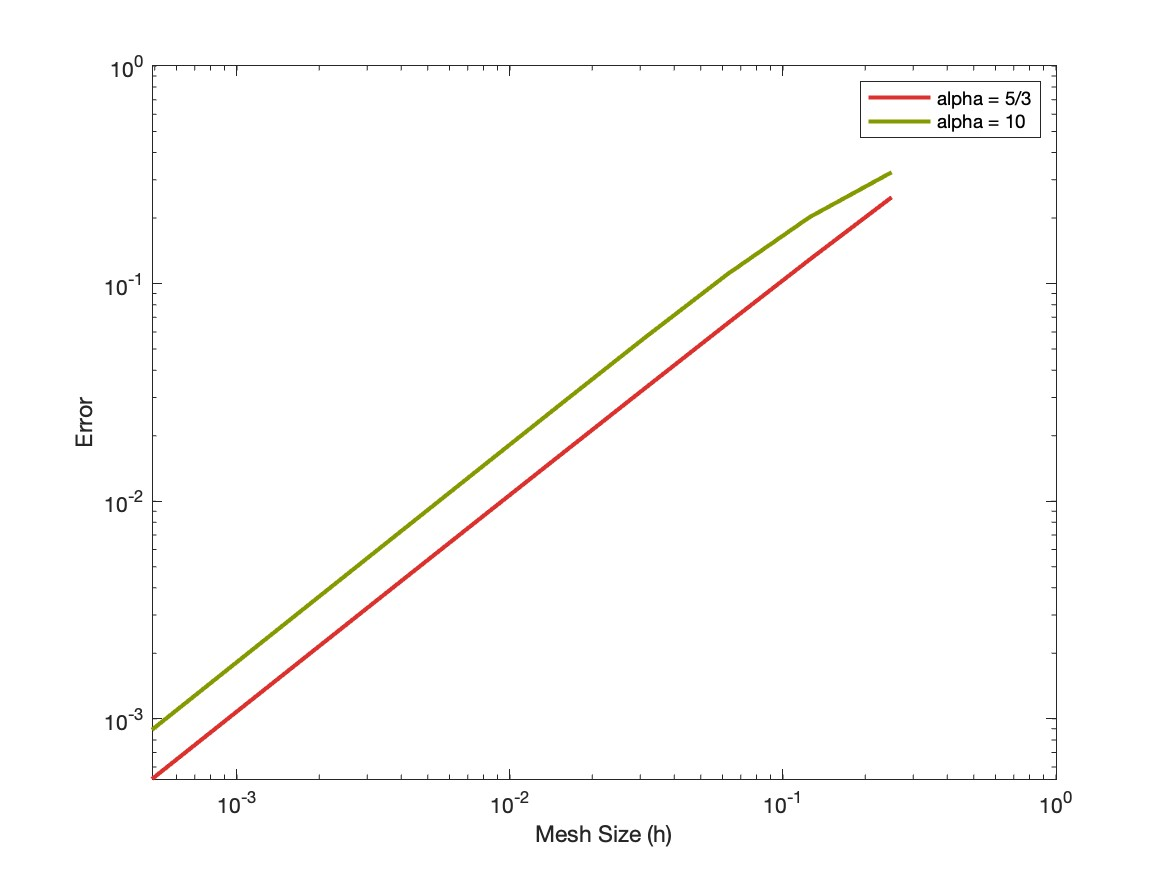
\includegraphics[width=15cm]{errorTrend.jpg}
	\caption{Error trend against mesh size for a sequence of uniform meshes.}
\end{figure}

\noindent Moreover a polynomial interpolation returns the following results which confirm the expected error trend on uniform meshes.
\begin{verbatim}
alpha = 5/3, y = 1.003215x + (-0.435934)
alpha = 10, y = 1.014542x + (-0.665838)
\end{verbatim}

	\newpage
	\section{Tests on Uniform Meshes}
	\subsection{Qualitative Comparison Between Analytical and Numerical Solution}

Here it follows a simple and qualitative comparison between the analytical and numerical solution on a single uniform mesh with $N_{el} = 2^{11}$.

\begin{figure}[!ht]
	\centering
	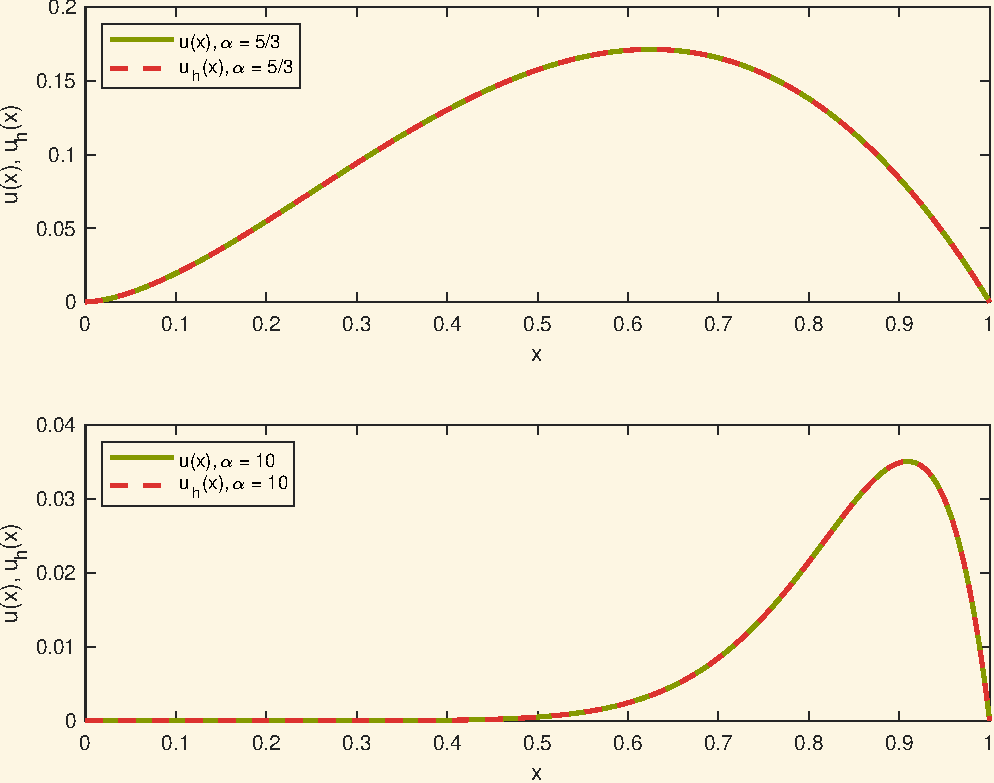
\includegraphics[width=15cm]{graphical.pdf}
	\caption{Qualitative comparison.}
\end{figure}

\subsection{FEM Convergence on Uniform Meshes}

Given what we've said on \nameref{sob_regularity}, and by the following corollary to the \textit{Deny-Lions' Lemma}:

\begin{theorem*}[Deny-Lions' corollary]
	Let $u, u_h$ be the solution respectively to the weak formulation of a Poisson problem and its associated order k Lagrangian FEM with shape-regular and quasi-uniform mesh $\Tau_h$. \\ 
	If $u \in H^s(\Omega)$, then $\exists C$ such that:
	\begin{gather}
		|u - u_h|_{1, \Omega} \le C (\max_{K \in \Tau_h} h_K)^{p}|u|_{s+1, \Omega},
	\end{gather}
	with $p = \min(s, k)$.
\end{theorem*}

Having defined a 1st-order Lagrangian FEM, we have for both values of $\alpha$ that $p = 1$, so that\footnote{The value of $s$ depends on the value of $\alpha$. We can always choose $s > k$.}:
\begin{gather}
	|u - u_h|_{1, \Omega} \le C (\max_{K \in \Tau_h} h_K)|u|_{s+1, \Omega}.
\end{gather}

By\footnote{For an appropriate choice of $s$.}:
\begin{gather}
	\max_{K \in \Tau_h} h_K = h, \\
	|u|_{s+1, \Omega} < +\infty,
\end{gather}
we have:
\begin{gather}
	|u - u_h|_{1, \Omega} \le C_1 h.
\end{gather}

\begin{figure}[!ht]
	\centering
	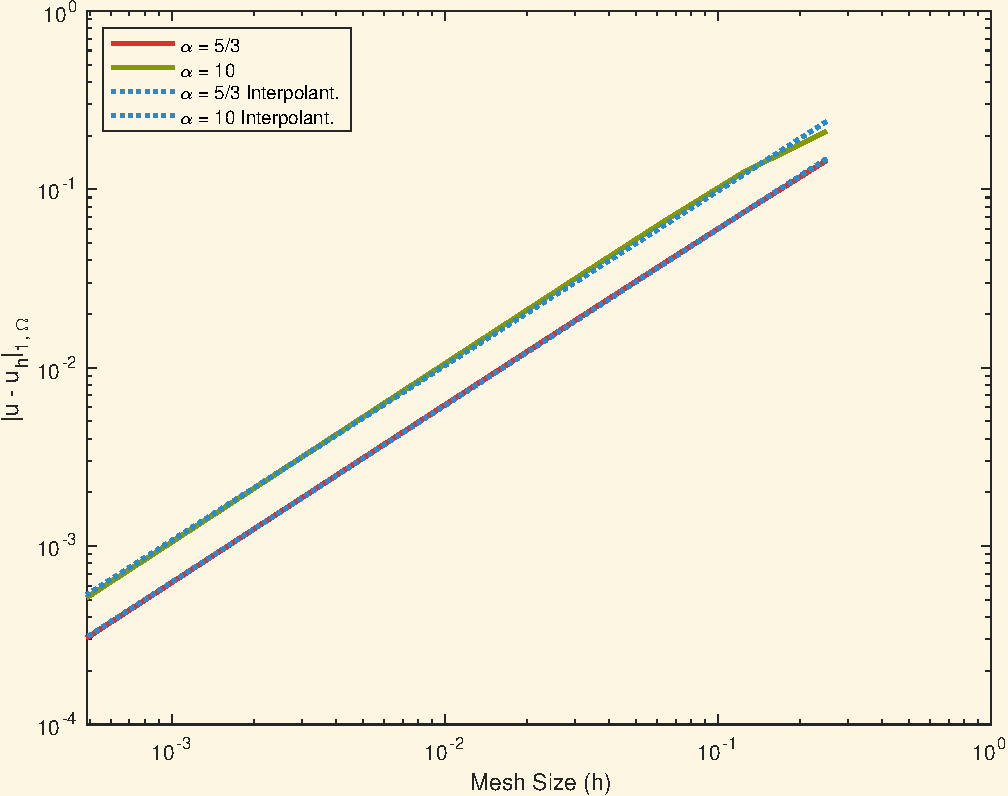
\includegraphics[width=15cm]{errorTrend.pdf}
	\caption{Error trend against mesh size for a sequence of uniform meshes.}
\end{figure}

\newpage
\noindent Moreover a polynomial interpolation returns the following results which confirm the expected error trend on uniform meshes, as they are decreasing slightly slower than linearly\footnote{This is a polynomial interpolation over a loglog relation which we use to return the polynomial order.}.

\lstinputlisting{../results/errorTrend.txt}

\newpage
\subsection{Stiffness Matrix Conditioning} \label{condition}

We want to investigate here the relation between the mesh size and the stiffness matrix' condtion number, expressed as it follows:
\begin{gather}
	\chi(\underline{\underline{A}}) \approx h^{-2}.
\end{gather}

The test is pretty straightforward as it requires to just evaluate the stiffness matrix for different meshes varying just the mesh size.

\begin{figure}[!ht]
	\centering
	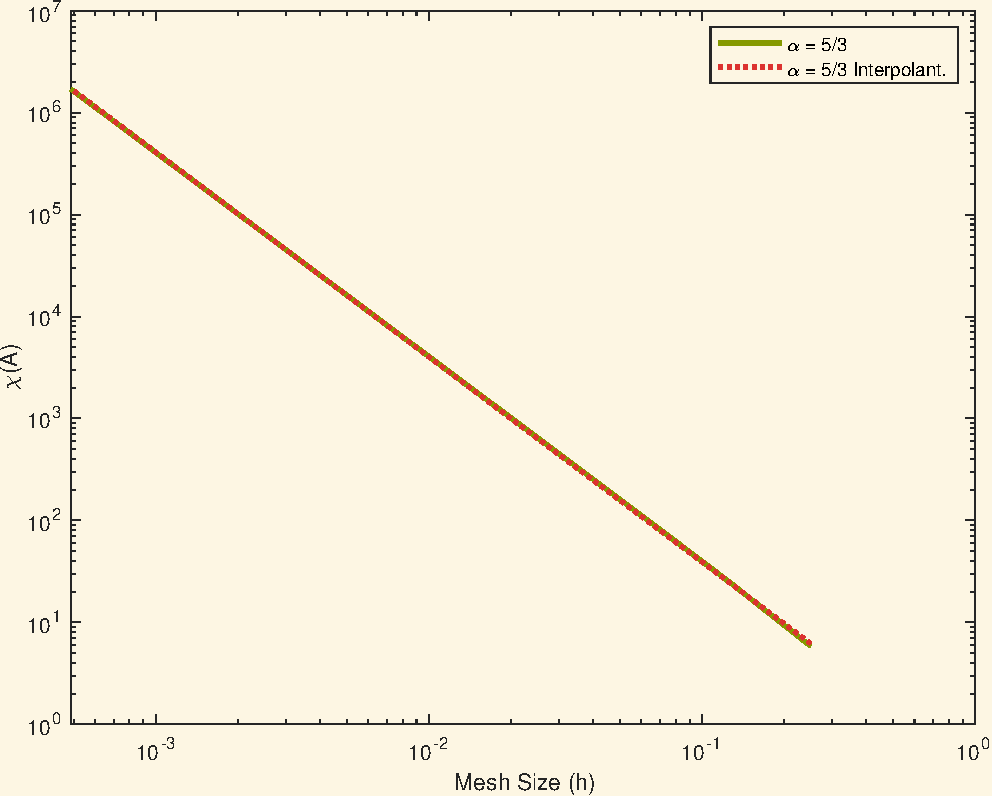
\includegraphics[width=15cm]{condition.pdf}
	\caption{Condition number against mesh size for a sequence of uniform meshes.}
\end{figure}

\newpage
\noindent Moreover a polynomial interpolation returns the following result which confirm the expected condition number trend\footnote{This is a polynomial interpolation over a loglog relation which we use to return the polynomial order.}.

\lstinputlisting{../results/condition.txt}

	\newpage
	\section{Adaptive Refinment Method}
	\subsection{Error Estimation and Refinement}

Instead of considering a sequence of uniformly refined meshes, we want to use a new algorithm that locally evaluates an error estimator and marks a certain number of elements for refinement. The local error estimator is given by:

\begin{gather} \label{estimator}
	\eta_K^2 = h_K \lVert f + \Delta u_h \rVert_{0, K}^2 + \frac{1}{2} \sum_{e \in E_K} h_K \lVert \llbracket \underline{\nabla} u_h \rrbracket \rVert_{0, e}.
\end{gather}

In the 1D case, we can rewrite \ref{estimator} as it follows\footnote{$K = [x_{n - 1}, x_n]$.}:

\begin{gather}
	\eta_K^2 = h_K \lVert f \rVert_{0, K}^2 + \frac{1}{2} h_K \left[ \lvert \llbracket u_h^\prime \rrbracket (x_{n - 1}) \rvert + \lvert \llbracket u_h^\prime \rrbracket (x_n) \rvert \right].
\end{gather}

To apply the algorithm, we evaluate $\eta_K$ for all elements $K \in \Tau_h$, and then select an arbitrary number of elements with the highest local error, e.g., the top 25\%, and mark them for refinement. The final step of the algorithm involves refining all the marked elements by adding a new node at their midpoint.

The algorithm can be summarized in the following steps:

\begin{description}
	\item[Solve] Solve the FEM problem on the \textit{starting mesh}.
	\item[Estimate] Estimate the local error for each element of the mesh.
	\item[Mark] Mark the elements with the highest local error (e.g., top 25\%).
	\item[Refine] Refine the marked elements by adding a new node at their midpoint.  
	\item[Repeat] Repeat the algorithm an arbitrary number of times. 
\end{description}

\newpage
\subsection{Reliability}

Let's test the results given by the following theorem on a sequence of uniformly refined mesh. This'll let us test the reliability of the error estimator $\eta$.

\begin{theorem*}[Reliability]
	Let $u \in H_0^1(\Omega)$ solution to the Poisson problem and $u_h$ solution to the Lagrangian FEM with a shape regular and quasi-uniform mesh $\Tau_h$. \\
	Then $\exists C$\footnote{$C$ depends only on the mesh $\Tau_h$.} such that:
	\begin{gather}
		\lvert u - u_h \rvert_{1, \Omega} \leq C \eta,
	\end{gather}
	where:
	\begin{gather}
		\eta^2 = \sum_{K \in \Tau_h} \eta_K^2.
	\end{gather}
\end{theorem*}

\begin{figure}[!ht]
	\centering
	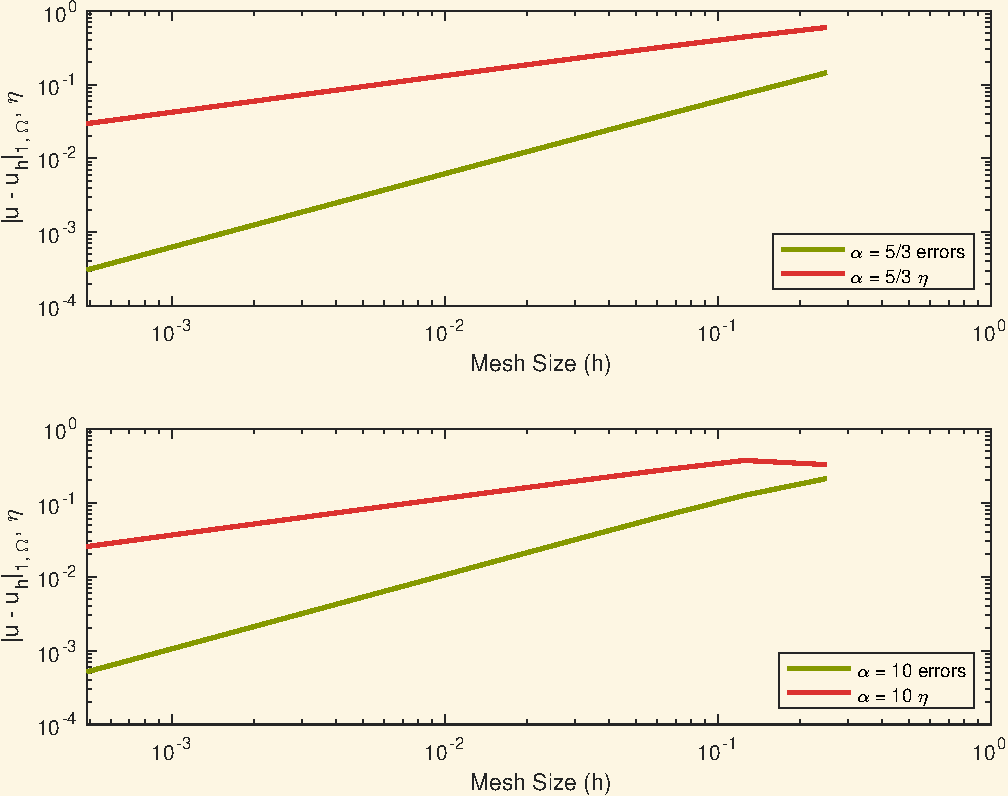
\includegraphics[width=15cm]{reliability.pdf}
	\caption{Comparison between errors and estimator against mesh size.}
\end{figure}

\newpage
\noindent Moreover we can obtain lower bounds for the constant $C$.

\lstinputlisting{../results/reliability.txt}

	\newpage
	\section{Comparisons}
\end{document}